\subsection{Edge Density Analysis}
This step analyzes edges using vertical Sobel operator from Gray-scale images. Figure \ref{fig:SobelResult1}, \ref{fig:SobelResult2}, and \ref{fig:SobelResult3} demonstrate the result we found after applying vertical Sobel filter on the original Gray-scale images.

\begin{figure}
\begin{subfigure}{0.5\textwidth}
    \centering
    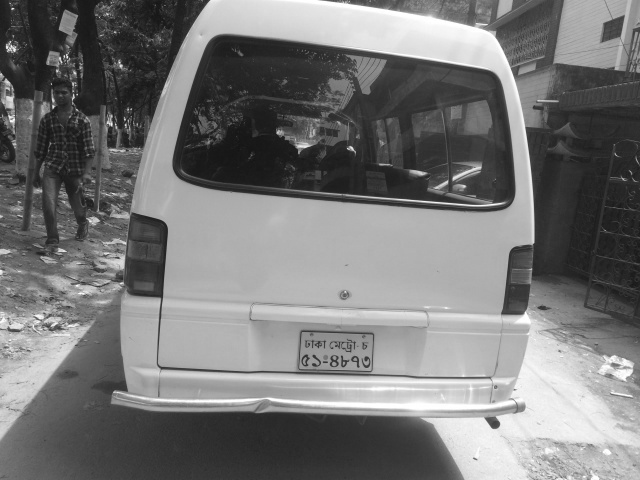
\includegraphics[width=0.9\linewidth]{./img/experiment/stage.2/angle}
    \caption{Original image}
\end{subfigure}
\begin{subfigure}{0.5\textwidth}
    \centering
    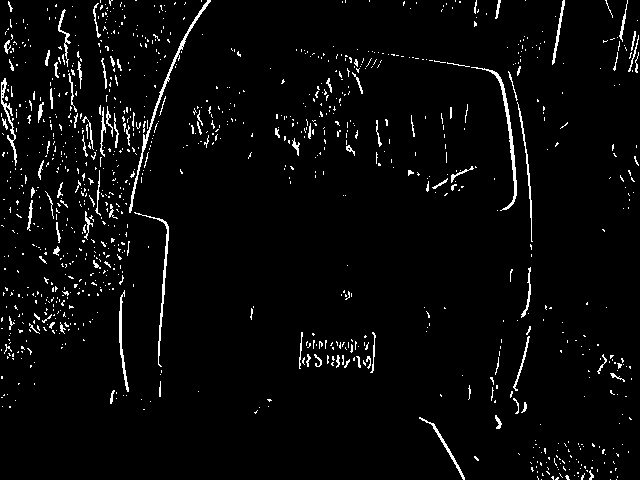
\includegraphics[width=0.9\linewidth]{./img/experiment/stage.3/angle}
    \caption{Edge image}
\end{subfigure}
\caption{Sobel image of a car with a slightly angled plate}
\label{fig:SobelResult1}
\end{figure}

\begin{figure}
\begin{subfigure}{0.5\textwidth}
    \centering
    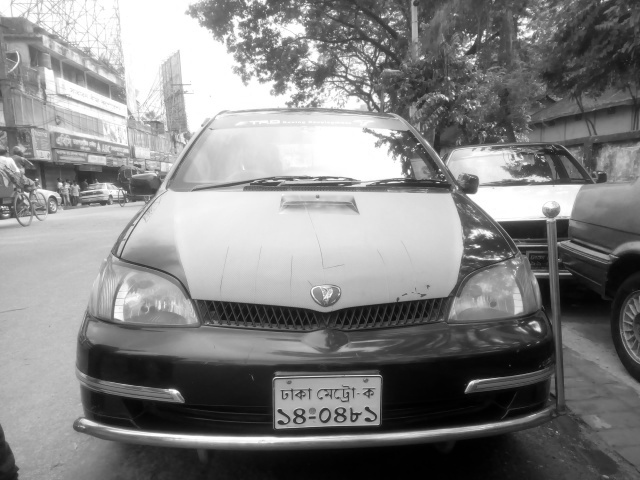
\includegraphics[width=0.9\linewidth]{./img/experiment/stage.2/good3}
    \caption{Original image}
\end{subfigure}
\begin{subfigure}{0.5\textwidth}
    \centering
    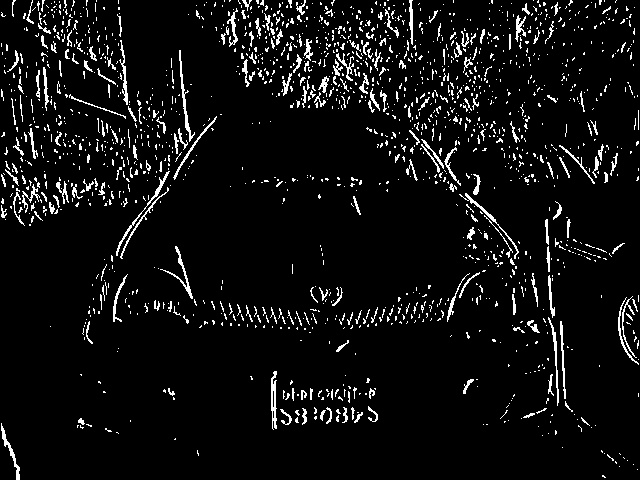
\includegraphics[width=0.9\linewidth]{./img/experiment/stage.3/good3}
    \caption{Edge image}
\end{subfigure}
\caption{Sobel image of a good plate image}
\label{fig:SobelResult2}
\end{figure}


\begin{figure}
\begin{subfigure}{0.5\textwidth}
    \centering
    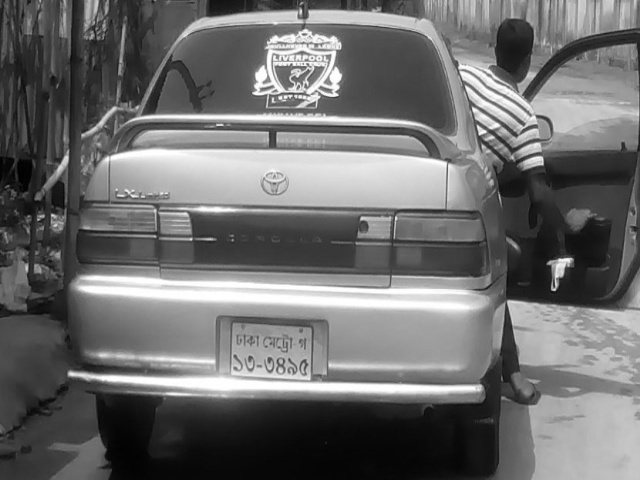
\includegraphics[width=0.9\linewidth]{./img/experiment/stage.2/light}
    \caption{Original image}
\end{subfigure}
\begin{subfigure}{0.5\textwidth}
    \centering
    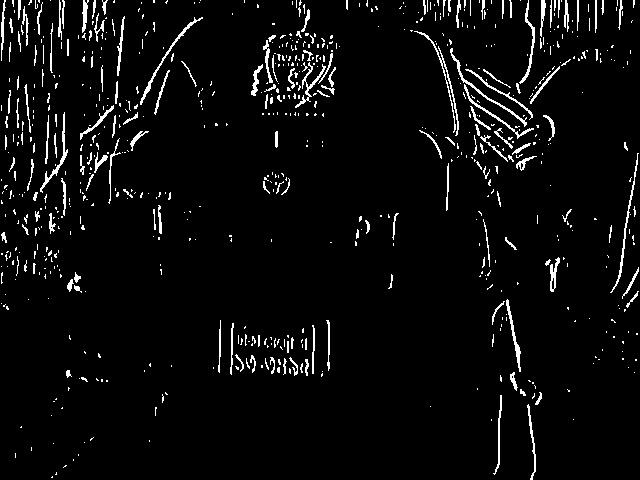
\includegraphics[width=0.9\linewidth]{./img/experiment/stage.3/light}
    \caption{Edge image}
\end{subfigure}
\caption{Sobel image of plate with light reflection}
\label{fig:SobelResult3}
\end{figure}
